%! TeX program = lualatex
\documentclass[../main.tex]{subfiles}
\begin{document} \section{Implicit differentiation}
  We learn the full picture of implicit differentiation in two steps. Step one is about the procedure. Step two is about the geometry.

  \begin{mdframed}[style=simple-compact]
    \textbf{The procedure}. To apply implicit differentiation to an \hlwarn{equation involving \(x,y\)} to find \(\tfrac{dy}{dx}\), we \hlwarn{assume} \hlmain{\(y\) is implicitly defined as a function of \(x\)} and do the following:
    \begin{enumerate}
      \item Differentiate \hlmain{both sides} of the equation \hlmain{with respect to \(x\)}, then
      \item \hlmain{Isolate} for \(\tfrac{dy}{dx}\) by treating \(\tfrac{dy}{dx}\) as a single symbol.
    \end{enumerate}

    The resulting \(\tfrac{dy}{dx}\) is a function in two variables \(x\) and \(y\). 
  \end{mdframed}

  \begin{example} \label{ex:implicit-circle}
    Use implicit differentiation to find \(\tfrac{dy}{dx}\) given \(x^{2} + y^{2} = 25\). 

    \begin{enumerate}[wide]
      \item Differentiate both sides with respect to \(x\) to get an equation in which \(\tfrac{dy}{dx}\) appears.
        \blanklines{10}

      \item Isolate for \(\tfrac{dy}{dx}\) to get \(\tfrac{dy}{dx} = \left( \cdots \text{ no } \tfrac{dy}{dx} \text{ here } \cdots \right)\).
        \blanklines{10}
    \end{enumerate}
  \end{example}

  \begin{example}
    Use implicit differentiation to find \(dy/dx\) given \(x = e^{y}\). 

    \blanklines{10}
  \end{example}

  \clearpage
  The Leibniz notation tells us which symbols is the function and which is the variable.
  \begin{example}
    Use implicit differentiation to find \(dx/dt\) given \(x^{3} - xt = 1\).  

    \blanklines{20}
  \end{example}

  Here is a more complicated example. Keep your writing well-organized to avoid little mistakes.
  \begin{example}
    Use implicit differentiation to find \(dy/dx\) given \(x^{2}y - \sin(xy) = 0\).

    \blanklines{25}
  \end{example}

  \clearpage
  \textbf{The geometric meaning}. Implicit differentiation allows us to find slopes of lines tangent to \hlwarn{curves} that are not functions. 

  Let's continue from Example~\ref{ex:implicit-circle}. Notice \(x^{2} + y^{2} = 25\) defines a curve. If we ``zoom in enough'' at a point on the curve and see a function, then \(\tfrac{dy}{dx}\) is the slope of the tangent line at that point. 

  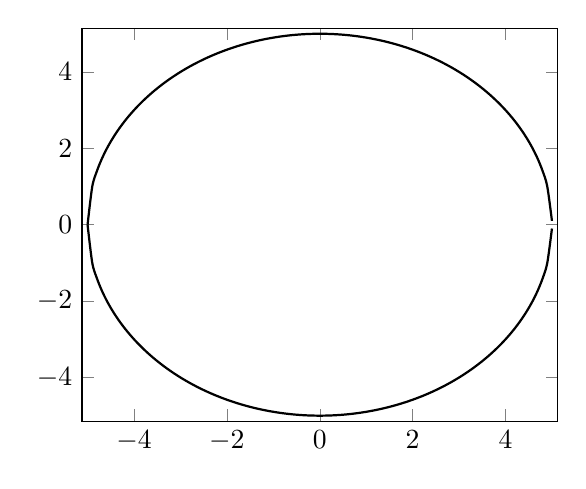
\begin{tikzpicture}[scale=1]
    \begin{axis}[smooth, samples=100, enlargelimits={abs=2pt}, width=3in, xmin=-5, xmax=5, ymin=-5, ymax=5]
      \addplot[thick, domain=-5:5] {sqrt(25 - x^2)};
      \addplot[thick, domain=-5:5] {-sqrt(25 - x^2)};
    \end{axis}
  \end{tikzpicture}
  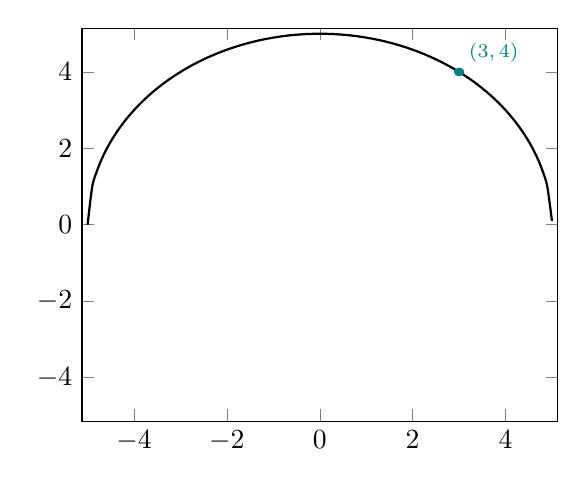
\begin{tikzpicture}[scale=1]
    \begin{axis}[smooth, samples=100, enlargelimits={abs=2pt}, width=3in, xmin=-5, xmax=5, ymin=-5, ymax=5]
      \addplot[thick, domain=-5:5] {sqrt(25 - x^2)};
      \draw[teal, fill] (axis cs:3,4) circle[radius=0.1] node[above right, teal] {\scriptsize \((3,4)\)};
    \end{axis}
  \end{tikzpicture}
  \begin{tikzpicture}[scale=1]
    \begin{axis}[smooth, samples=100, enlargelimits={abs=2pt}, width=3in, xmin=-5, xmax=5, ymin=-5, ymax=5]
      \addplot[thick, domain=4:5] {sqrt(25 - x^2)};
      \addplot[thick, domain=4:5] {-sqrt(25 - x^2)};
      \draw[magenta, fill] (axis cs:5,0) circle[radius=0.1] node[above left, magenta] {\scriptsize \((5,0)\)};
    \end{axis}
  \end{tikzpicture}

  \begin{example}
    Find an equation of the tangent line to the curve \(x^{2} + y^{2} = 25\) at \((3,4)\).
    \blanklines{20}
  \end{example}

  \faComment{} Can we use find the slope of the tangent line to the curve \(x^{2} + y^{2} = 25\) at \((5,5)\).
  \blanklines{10}

  \clearpage
  Here is an example tying together the procedure and the geometric meaning of implicit differentiation.
  \begin{example}
    Find an equation of the line tangent to the curve \(\tan(xy) = -x\) at the point \((1,3\pi/4)\).
    \blanklines{45}
  \end{example}

\end{document}
